\documentclass{article}
\usepackage[top=0pt,left=0pt,bottom=0pt,right=0pt,paperwidth=2.15cm,paperheight=6.7mm]{geometry}
\usepackage{tikz}
\pagestyle{empty}
\begin{document}
\centering%
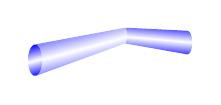
\begin{tikzpicture}
\coordinate (a) at (0,0);
\coordinate (b) at (170:8mm);
\path (b) ++(200:1.2cm) coordinate (c);

\path (a) arc(-95:90:0.6mm and 1.5mm) coordinate (a');
\path (b) arc(-90:90:0.2mm and 1mm) coordinate (b');
\path (c) arc(-80:-270:0.9mm and 2mm) coordinate (c');

\path[clip,rounded corners=1pt] (a) -- (b) -- (c) arc(-80:-265:0.9mm and 2mm) -- (b') -- (a') arc(90:-95:0.6mm and 1.5mm);
\begin{scope}
\path[clip] (a) -- (b) arc(-90:90:0.2mm and 1mm) -- (a') arc(90:-95:0.6mm and 1.5mm);
\shade [top color=blue, bottom color=blue,middle color=white,shading angle=-5] ([xshift=5pt]a) rectangle ([yshift=1pt]b');
\end{scope}

\begin{scope}
\path[clip] (b) -- (c) arc(-80:100:0.9mm and 2mm) -- (b') arc(90:-90:0.2mm and 1mm);
\shade [top color=blue, bottom color=blue,middle color=white,shading angle=15] ([xshift=1pt,yshift=3pt]b') rectangle ([yshift=-1pt,xshift=-1pt]c);
\end{scope}

\begin{scope}
\path[clip] (c) arc(-80:280:0.9mm and 2mm);
\shade [top color=blue, bottom color=blue,middle color=white,shading angle=15] ([xshift=3pt,yshift=1pt]c') rectangle ([yshift=-1pt,xshift=-3pt]c);
\end{scope}
\end{tikzpicture}
\end{document}
